\documentclass[10pt,a4paper]{article}
\usepackage[utf8]{inputenc}
\usepackage[english]{babel}
\usepackage{amssymb,amsfonts, amsmath, textcomp}
\usepackage{calc}
\usepackage{ifthen}
\usepackage{graphicx}
\usepackage{listings, color}
\usepackage{url}
\linespread{1.5}

\definecolor{dkgreen}{rgb}{0,0.45,0}
\definecolor{gray}{rgb}{0.5,0.5,0.5}
\definecolor{mauve}{rgb}{0.30,0,0.30}

% Default settings for code listings
\lstset{frame=tb,
  language=Java,
  aboveskip=3mm,
  belowskip=3mm,
  showstringspaces=false,
  columns=flexible,
  basicstyle={\small\ttfamily},
  numbers=left,
  numberstyle=\footnotesize,
  keywordstyle=\color{dkgreen}\bfseries,
  commentstyle=\color{gray},
  stringstyle=\color{mauve},
  frame=single,
  breaklines=true,
  breakatwhitespace=true,
  tabsize=1
}

\title{\rule{12.5cm}{0.5mm}\\Advanced Algorithms in Computational Biology\\DM845}
\author{Martin Østergaard Villumsen\\\texttt{mvill11@student.sdu.dk}\\\rule{6.5cm}{0.5mm}\\University of Southern Denmark\\}
\date{\today}

\begin{document}
\maketitle
\newpage

\section{Introduction}
The human genome is diploid which means that each cell has two homologous copies of each chromosome, one from the mother and one from the father. In order to understand the genetic basis for different diseases (e.g. cancer) it is not sufficient to detect the SNPs, we also need to assign each SNP to the two copies of the chromosome and current methods for doing so suffers from the fact that the reads are too short \cite{whatshap}.

In this project we will develop a simple read simulator, which generates reads that are much longer than those obtained from e.g. Next-Gen sequencing machines. We will simulate reads with different parameters such as read length and sequencing error probability and assign SNPs to each chromosome from these reads using \textsc{WhatsHap}, a novel dynamic programming approach to haplotype assembly described in \cite{whatshap}. We will then evaluate the results and compare them with those presented in \cite{whatshap}.

\subsection{Biological Problem}
The task of assigning SNPs to a concrete chromosome is called phasing and the resulting groups of SNPs are called haplotypes. We need to discover and phase all these SNPs in order to gain a better understanding for e.g. some diseases by linking possibly disease-causing SNPs with one another. By doing so we can reconstruct haplotypes from a collection of sequenced reads which is known as haplotype assembly.

\subsection{Computational Problem}
There are two groups of single nucleotide variants: Those that are homozygous and those that are heterozygous. Individuals that are homozygous at every locus or heterozygous at just one locus can easily be phased, however, if we have $m$ heterozygous SNPs, there are $2^m$ possible haplotypes which illustrates that it is a hard computational problem. Therefore we are only concerned with heterozygous SNPs when doing haplotype assembly. 

What also makes this a computational hard problem is the fact that we want to phase an reconstruct the haplotypes directly from sequencing reads. 

\section{Haplotype Assembly with WhatsHap}
There are two major approaches to phasing variants: One approach relies on genotypes as input along with the zygosity status of the SNPs, and the other approach phases directly from sequencing read data \cite{whatshap}. \textsc{WhatsHap} belongs to the latter. 

\textsc{WhatsHap} has been developed with the parsimony principle in mind, i.e. computing two haplotypes to which we can assign all reads while minimizing the amount of sequencing errors to be corrected or removed \cite{whatshap}. This resembles the minimum error correction (MEC) problem which consists of finding the minimum number of corrections to the SNP values to be made to the input in order to be able to arrange the reads into two haplotypes without conflicts \cite{whatshap}. This can easily be adapted to a weighted version of the problem, namely the weighted minimum error correction problem (wMEC). The weight in this case reflects the relative confidence that a single nucleotide is correctly sequenced.

Even though the wMEC problem is NP-hard \textsc{WhatsHap} creates an exact solution to the problem in linear time. This is done by the use of dynamic programming and assuming a bounded coverage, i.e. the implementation can solve the problem in linear time on datasets of maximum coverage up to 20x \cite{whatshap}. The algorithm is a fixed parameter tractable approach to the wMEC where the running time is only depending on the coverage, i.e. the number of reads that cover a SNP position.

The input to the wMEC problem is a matrix with entries $\in\{0, 1, -\}$ where each row corresponds to a read and each column corresponds to a SNP position. Each entry is associated with a weight telling how likely it is that the entry is correctly sequenced. We want to find a minimum weight solution and when these weights are log-likelihoods, summing them up corresponds to multiplying probabilities, thus finding the minimum weight solution corresponds to finding a maximum likelihood bipartition of the reads \cite{whatshap}. And this is basically what the authors of \textsc{WhatsHap} is using a dynamic programming approach to do. By using this approach they find an optimal solution to the wMEC problem for each column of the matrix and then an optimal bipartition of the reads can be obtained by backtracking along the columns of the dynamic programming table. For further details see \cite{whatshap}.


% Description of algorithms/methods used
% Links to papers/data/software etc.
% Description of data
\section{Building a DNA Simulator}
% My contributions
\section{Results and Discussion}
%% TODO: List of commands to recreate my results.

\begin{figure}[h!]
\centering
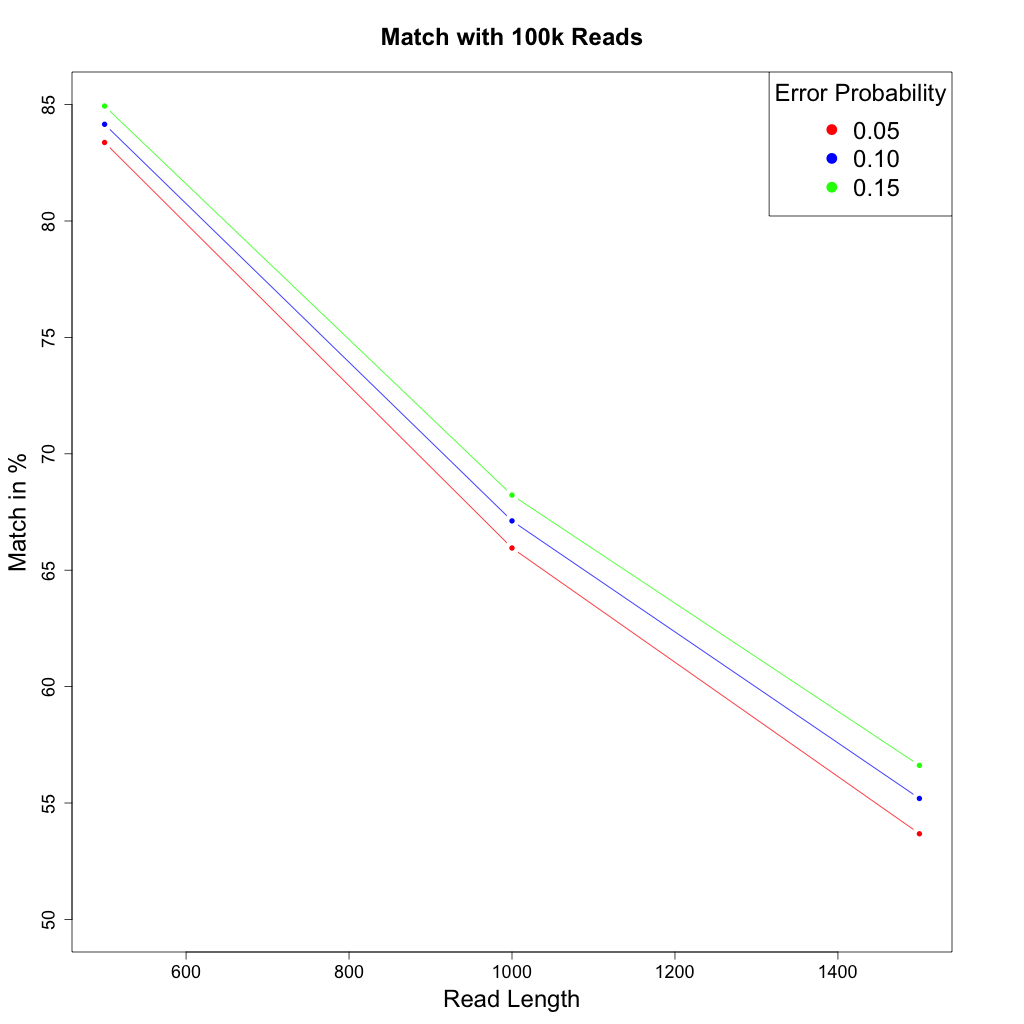
\includegraphics[width=\textwidth]{../output/plots/plot100k}
\caption{Results of haplotype assembly of 100.000 reads}
\end{figure}
\begin{figure}[h!]
\centering
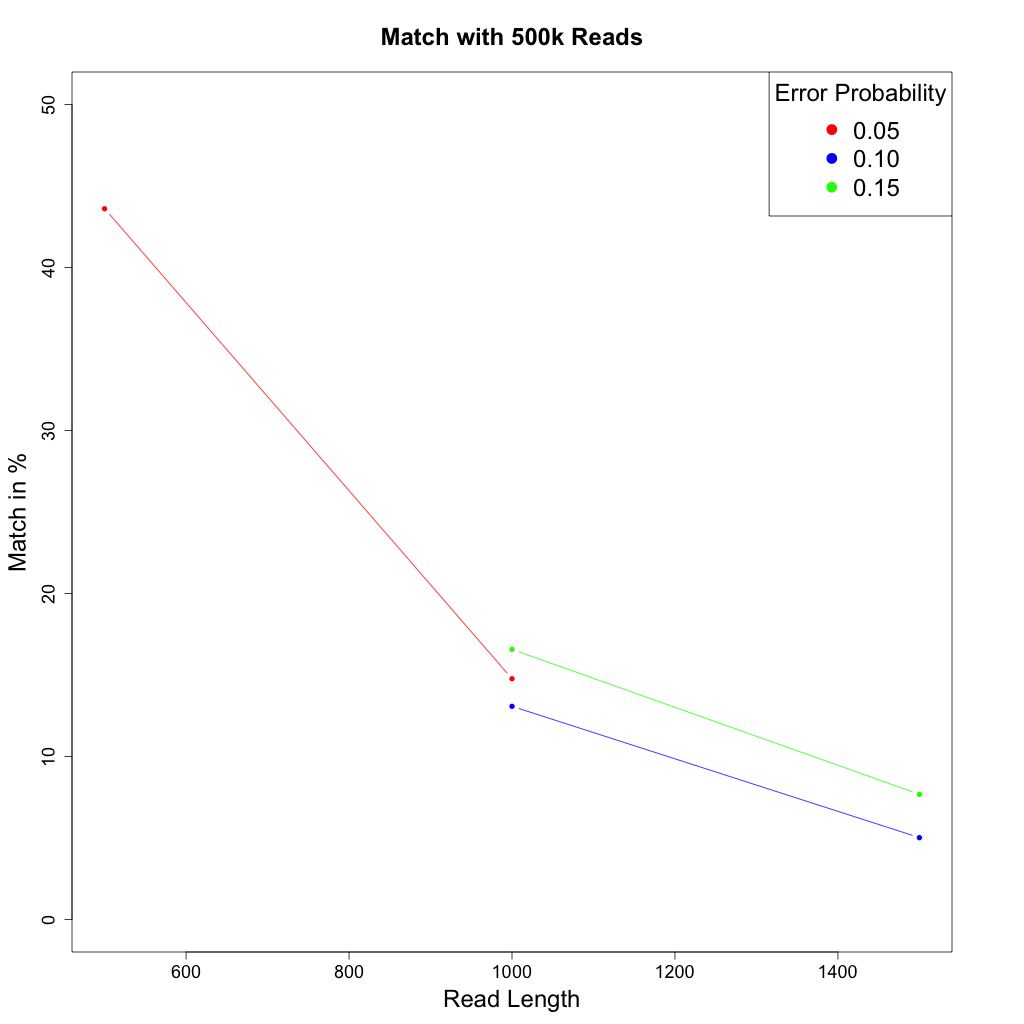
\includegraphics[width=\textwidth]{../output/plots/plot500k}
\caption{Results of haplotype assembly of 500.000 reads}
\end{figure}

\begin{figure}[h!]
\centering
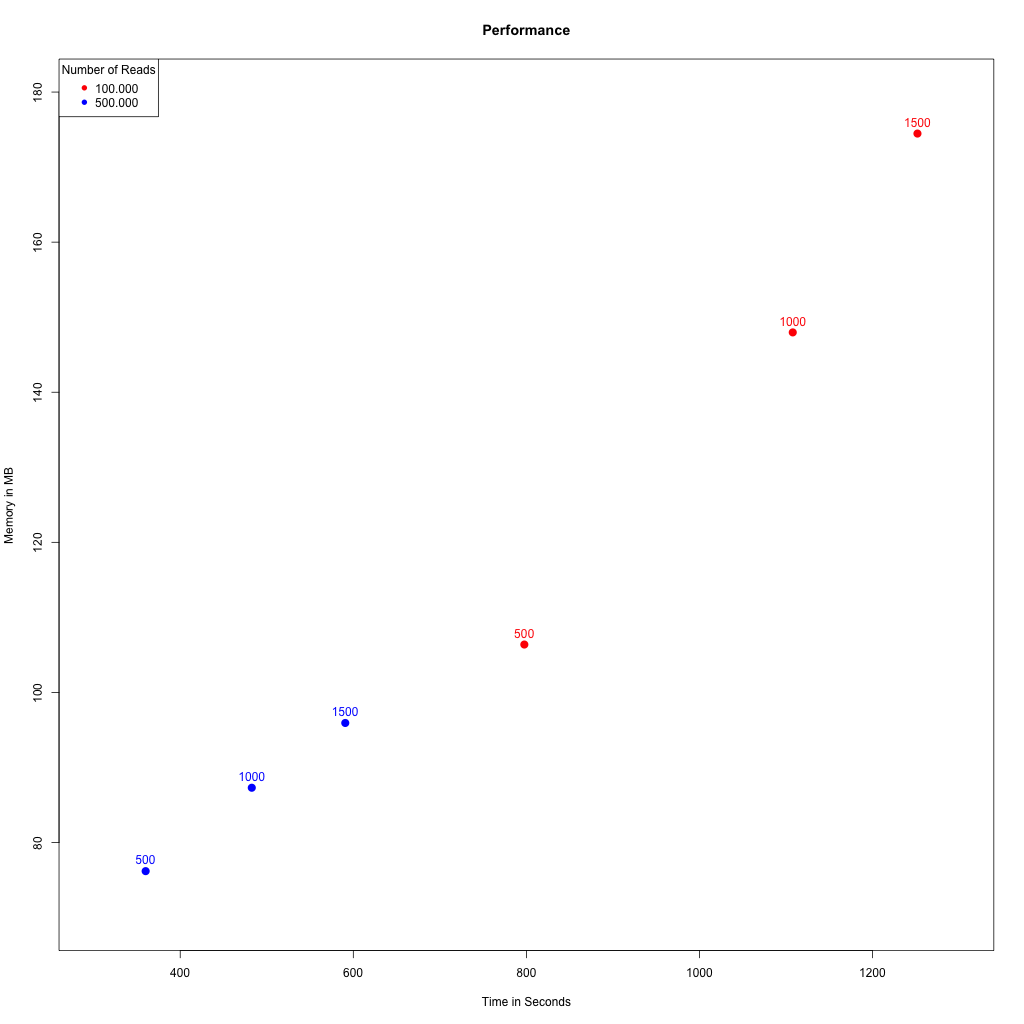
\includegraphics[width=\textwidth]{../output/plots/plotPerformance}
\caption{Performance}
\end{figure}

\section{Conclusion}
% Length of chrm1: 230.481.193
\addcontentsline{toc}{section}{References}
\bibliography{whatshap}{}
\bibliographystyle{abbrv}
\end{document}
